\documentclass[12pt]{article}
\usepackage{graphicx} % Required for inserting images
\usepackage{enumitem}
\usepackage{amsmath}
\usepackage{gvv-book}
\usepackage{gvv}

\title{\textbf{2.7.16}}
\author{\textbf{EE25BTECH11004 - Aditya Appana}}
\date{August 30, 2025}

\begin{document}

\maketitle

\section*{Question}
Find $|\vec{a}\times \vec{b}|$ if $\vec{a} = (2\hat{i} +\hat{j} +3\hat{k})$ and  $ \vec{b}=(3\hat{i} + 5\hat{j} - 2\hat{k})$

\section*{Solution}
The vectors are
\begin{align} 
\vec{a} = \myvec{2\\1\\3}\\
\vec{b} = \myvec{3\\5\\-2}
\end{align}

To calculate the cross-product of the two vectors \vec{a} and \vec{b}, we use the following determinant:
$$\myvec{|\vec{A_{23}} \vec{B_{23}}| \\ |\vec{A_{31}}   \vec{B_{31}}| \\ |\vec{A_{12}} \vec{B_{12}}| }$$


Where $\vec{X_{ij}} = \myvec{$x_i$ \\ $x_j$}$ 

\newpage

Expanding the determinants, we get: 
\begin{align}
\myvec{ ((-2) - 15) \\ ((-4) - 9) \\ (10-3)}  \\
= \myvec{-17\\13\\7}
\end{align}

We need to find the norm of this vector, which is done by:
\begin{align}
\sqrt{17^2+13^2+7^2} \\
=22.516660498395403
\end{align}

\vspace{0.5cm}


\begin{figure}[H]
    \centering
    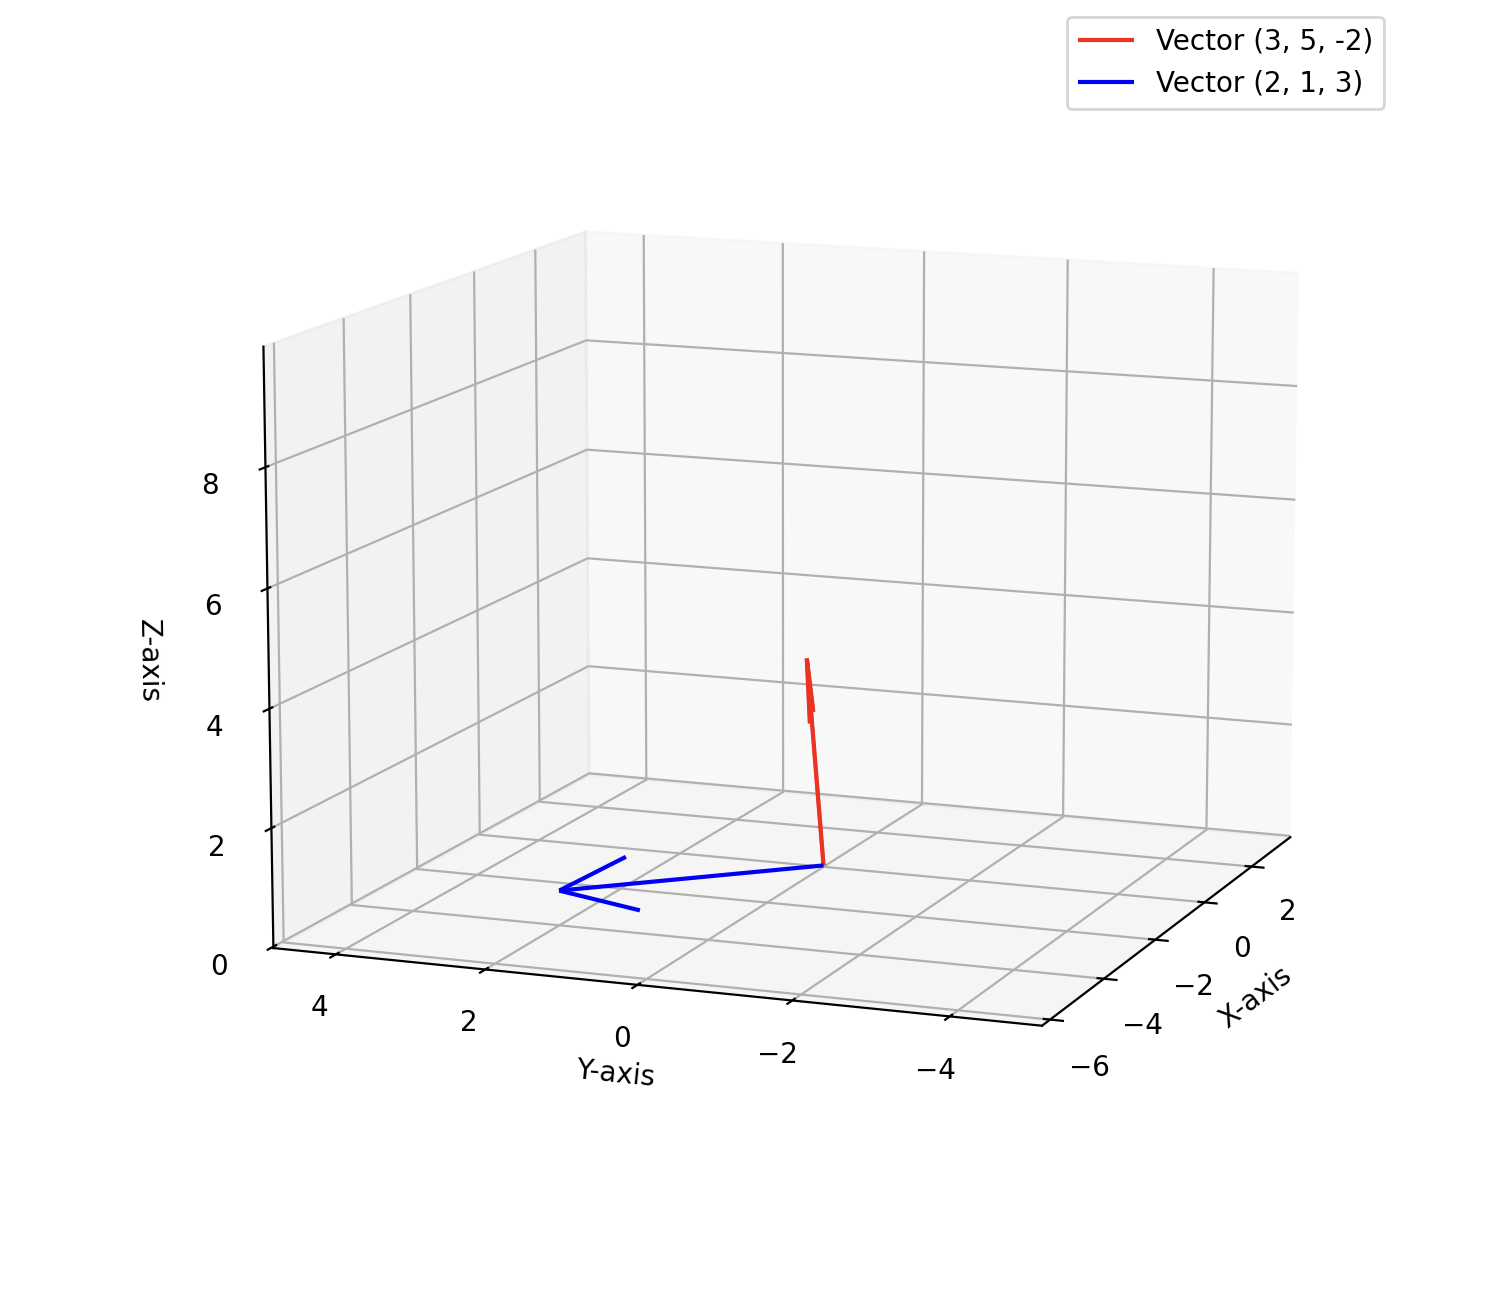
\includegraphics[width=0.7\columnwidth]{Figs/Figure_4.png}
    \caption{Plot}
    \label{fig:placeholder}
\end{figure}

\end{document}